\section{Complexity}

This section defines the measures which should be computed with the analysis.
Therefore, we introduce the terms of time, size and cost complexity.
Time complexity describes how many steps an evaluation of a program will take in a worst-case scenario.
Size complexity yields for each transition an assignment from each variable to an interval, which defines the range of the value of the variable after the execution of the transition in an arbitrary run.
The third type is cost complexity.
While the costs of a transition are not considered in the time complexity, the cost complexity considers the costs of transitions and describes the cost of the sequence of transitions taken in a worst-case run.
Time complexity can be seen as a special case of cost complexity, where the cost $c(t)$ of every transition $t \in \TSet$ equals $1$.

\subsection{Time Complexity}

We define the time complexity of a program $\Program$ as the highest possible number of steps in an arbitrary run with an initial state $\valuation_0 \in \Valuation$ between a lower and an upper bound $\lstate \leq \valuation_0 \leq \ustate$.

\begin{definition}[Worst-Case Time Complexity]
  We call $\text{rc}: (\Valuation \times \Valuation) \rightarrow \mathbb{N}$ the \textbf{time complexity} of a program if and only if for all states $\lstate, \ustate \in \Valuation$ it holds that
  \[ \text{rc}(\lstate, \ustate) = \timecomplexityterm \]
\end{definition}

An upper time bound of a transition $t \in \TSet$ describes a maximal number of occurrences of that transition in an evaluation starting with an arbitrary initial state $\valuation_0 \in \Valuation$ between a lower and an upper bound $\lstate \leq \valuation_0 \leq \ustate$.

\begin{definition}[Upper Time Bound]
  We call $\UTime: \TSet \rightarrow \BoundSet(\PVSet)$ an \textbf{upper time bound} if and only if for all $t \in \TSet$ and all states $\lstate, \ustate \in \Valuation$ it holds that
  \[ \ueval{\UTime(t)}{\lstate}{\ustate} \geq \timeboundterm \]
  We also refer to an upper time bound as \textbf{time bound}, since lower time bounds are not considered in this thesis.
\end{definition}

In the KoAT paper \cite{koat} a different definition of time complexity is used.
Note that while the KoAT paper uses input vectors in $\mathbb{N}^{\abs{\PVSet}}$, we use an equivalent representation with states in $\Valuation$.
Then, $\text{rc}'(m) = \sup \braced{ k \in \mathbb{N} \mid \exists \valuation_0, \location, \valuation: \abs{\valuation_0} \leq m \wedge (\location_0, \valuation_0) \rightarrow^k (\location, \valuation) }$ is an equivalent representation of the defined time complexity of the KoAT paper, if the input state $m \in \Valuation$ is defined with $m(v) \geq 0$ for all variables $v \in \PVSet$.
We can show, that this definition is a special case of the new definition of time complexity.

\begin{remark}[Original KoAT time complexity]
  Let $-\valuation$ denote the negation $(-\valuation)(v) := -\valuation(v)$ of the value of every variable $v \in \PVSet$ for a state $\valuation$.
  Let $\text{rc}'(m) = \sup \braced{ k \in \mathbb{N} \mid \exists \valuation_0, \location, \valuation: \abs{\valuation_0} \leq m \wedge (\location_0, \valuation_0) \rightarrow^k (\location, \valuation) }$ be the time complexity definition of the original KoAT.
  Then, for every state $m \in \Valuation$ it holds that
  \[ \text{rc}'(m) = \text{rc}(-m,m). \]
\end{remark}

Therefore, if only the information is given, that for an input state $\valuation \in \Valuation$ it holds that $-m \leq \valuation \leq m$, the time complexity $\text{rc}'(m)$ of the original KoAT paper and the new time complexity $\text{rc}(-m,m)$ yield the same result.
But if the information is given, that for an input state $\valuation$ it holds that $\lstate \leq \valuation \leq \ustate$, the new time complexity $\text{rc}(\lstate, \ustate)$ can use this information.
With the original definition it is necessary to define an input state $m$ with $m(v) = \max(\abs{\lstate(v)}, \abs{\ustate(v)})$ for each variable $v \in \PVSet$ to gain a time complexity $\text{rc}'(m)$.
Therefore, the additional information $\lstate \leq \valuation \leq \ustate$ is not utilized in the original definition, resulting in a time complexity $\text{rc}'(m)$ greater or equal than $\text{rc}(\lstate, \ustate)$.
Thus, the time complexity $\text{rc}(\lstate, \ustate)$ is closer to the real time complexity of a program than the original time complexity.

\begin{example}[Comparison of time complexity definitions]
  Consider the program in Figure \ref{fig:motivational_example}.
  \begin{figure}
  \centering
  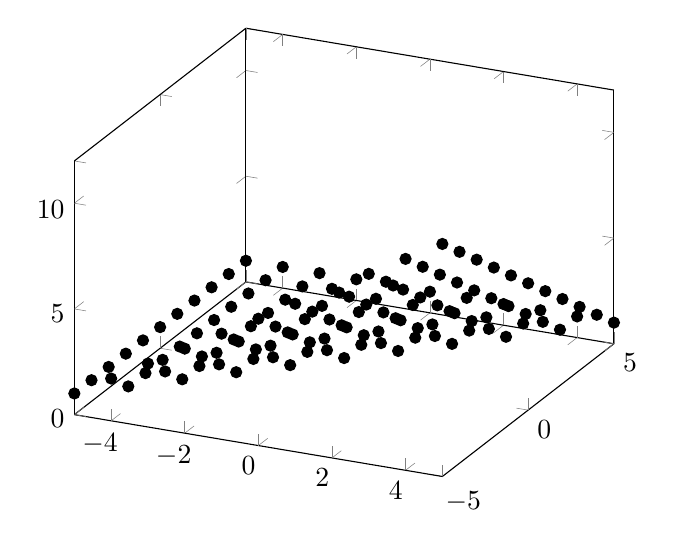
\begin{tikzpicture}
    \begin{axis}
      \addplot3 [
        unbounded coords=jump,
        mesh,
        shader=interp,
        samples at={-5,...,5},
        samples y={11},
        only marks,
      ] {1+max(x-y,0)};
    \end{axis}
  \end{tikzpicture}
  \hfil
  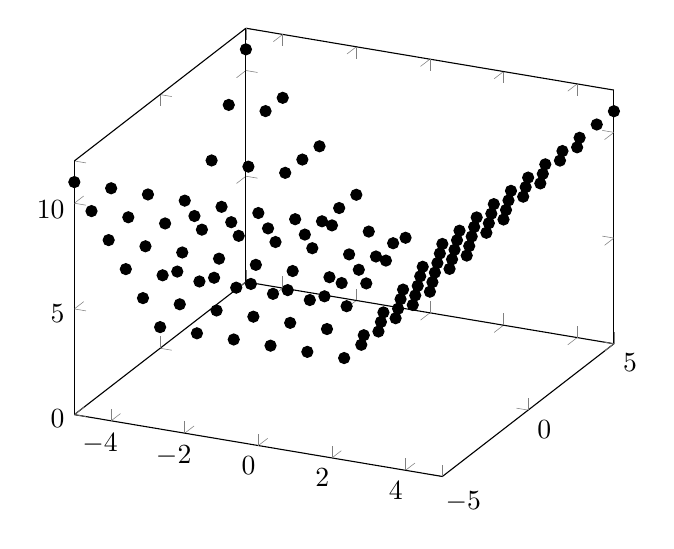
\begin{tikzpicture}
    \begin{axis}
      \addplot3 [
        unbounded coords=jump,
        mesh,
        shader=interp,
        samples at={-5,...,5},
        samples y={11},
        only marks,
      ] {1+abs(max(x,-y))+abs(max(x,-y))};
    \end{axis}
  \end{tikzpicture}
  \caption{Evaluation of the motivational example}
  \label{fig:motivational_evaluation}
\end{figure}

  This program graph corresponds to the motivational program from the introduction.
  Let $\lstate, \ustate \in \Valuation$ be states with $\ustate(x) = 4$, $\ustate(y) = 2$, $\lstate(x) = -6$ and $\lstate(y) = 0$.
  An input state for the original KoAT would therefore be an $m \in \Valuation$ with $m(x) = \max(\abs{\lstate(x)}, \abs{\ustate(x)}) = \max(\abs{-6}, \abs{4}) = 6$ and $m(y) = \max(\abs{\lstate(y)}, \abs{\ustate(y)}) = \max(\abs{0}, \abs{2}) = 2$.
  The time complexity of the original KoAT would then be $\text{rc}'(m) = 9$, since with a state $\valuation'_0 \in \Valuation$ with $\valuation'_0(x) = 6$ and $\valuation'_0(y) = -2$ (and therefore $-6 \leq \valuation'_0(x) \leq 6$ and $-2 \leq \valuation'_0(y) \leq 2$) we have one occurrence of $t_0$ and eight occurrences of $t_1$.
  Since $\lstate \nleq \valuation'_0 \nleq \ustate$, the state $\valuation'_0$ is not a possible input state for the time complexity $\text{rc}$.
  Instead, the input state yielding the greatest numbers of evaluation steps is a state $\valuation_0 \in \Valuation$ with $\valuation_0(x) = 4$ and $\valuation_0(y) = 0$.
  Therefore, the new time complexity $\text{rc}(\lstate, \ustate)$ is $1 + 4$, which is significantly closer to the real time complexity than the time complexity of the original KoAT $\text{rc}'(m) = 9$.
\end{example}
  
Although we changed the definitions of time complexity and time bounds, the known theorem, that it is possible to approximate the time complexity of a program by the sum of all upper time bounds, is still valid.

\begin{theorem}[Approximating time complexity]
  Let $\UTime$ be a time bound for $\TSet$.
  Then, 
  \[ \text{rc} \leq \sum_{t \in \TSet}\UTime(t) \]
  holds.
\end{theorem}


Therefore, it is sufficient to determine an upper time bound for a program and build the sum over all transitions $\TSet$ of the program, to approximate the time complexity. 

\subsection{Size complexity}

For each variable at a particular transition, a size bound defines an interval in which the value ranges in a worst-case evaluation.
This interval is defined by a lower size bound and an upper size bound.
While upper size bounds are always greater than the greatest possible value at a transition, lower size bounds are always smaller than the lowest possible value.

\begin{definition}[Worst-Case Size Bound]
  Let $\RV = \TSet \cup \VSet$ be the set of all result variables.
  We call $\USize: \RV \rightarrow \BoundSet(\PVSet)$ an \textbf{upper size bound} if and only if for every result variable $(\actt, v) \in \RV$ and all states $\lstate, \ustate \in \Valuation$ it holds that
  \[ \ueval{\USize(\actt, v)}{\lstate}{\ustate} \geq \usizeboundterm. \]
  Furthermore, we call $\LSize: \RV \rightarrow \BoundSet(\PVSet)$ a \textbf{lower size bound} if and only if for every result variable $(\actt, v) \in \RV$ and all states $\lstate, \ustate \in \Valuation$ it holds that
  \[ \leval{\LSize(\actt, v)}{\lstate}{\ustate} \leq \lsizeboundterm. \]
  We call $\Size$ a \textbf{size bound}.
\end{definition}

Note that for a transition $t = (\location,\text{id},\guard,\location') \in \TSet$, the upper size bound $\USize(t,x) = x$ is identical to the lower size bound $\LSize(t,x) = x$.
Different upper and lower size bounds result from further restrictions on the incoming variables.
With $\guard = \braced{x \geq 0}$, we can determine $\USize(t,x) = x$ as an upper bound and $\USize(t,x) = 0$ as a lower bound.

The presented definition of size bounds expresses a bound depending on the values at the start of the program.
For the definition of the methods for the computation of trivial and nontrivial size bounds, we also need a definition of bounds depending on the values immediately before the execution of a transition.
These local size bounds can be lifted to global size bounds by the upcoming definitions of trivial and nontrivial size bounds.

\begin{definition}[Local Size Bound]
  We call $\ULSB: \RV \rightarrow \BoundSet(\PVSet)$ an \textbf{upper local size bound} if and only if for every result variable $(t, v) \in \RV$ and all states $\lstate, \ustate \in \Valuation$ it holds that
  \[ \ueval{\ULSB(t, v)}{\lstate}{\ustate} \geq \ulocalsizeboundterm. \]
  Furthermore, we call $\LLSB: \RV \rightarrow \BoundSet(\PVSet)$ a \textbf{lower local size bound} if and only if for every result variable $(t, v) \in \RV$ and all states $\lstate, \ustate \in \Valuation$ it holds that
  \[ \leval{\LLSB(t, v)}{\lstate}{\ustate} \leq \llocalsizeboundterm. \]
  We call $\LSB$ a \textbf{local size bound}.
\end{definition}

\begin{example}[Local Size Bound]
  \begin{figure}
\centering
\begin{tikzpicture}[->,>=stealth',auto,node distance=5cm,
    thick,
    main node/.style={circle,draw,font=\sffamily\Large\bfseries},
    aligned edge/.style={align=left}]

  \node[main node] (0) {$l_0$};
  \node[main node] (1) [right of=0] {$l_1$};
  \node[main node] (2) [right of=1] {$l_2$};

  \path[every node/.style={font=\sffamily\small}]
    (0) edge[aligned edge] node[above=0.2cm] {$t_0$} node[below=0.2cm] {$\update(x) = x + 1$} (1)
    (1) edge[aligned edge] node[above=0.2cm] {$t_1$} node[below=0.2cm] {$\update(x) = 2 \cdot x$} (2)
    ;
\end{tikzpicture}
\caption{Example for the difference between local and global effects}
\label{fig:localglobal}
\end{figure}

  Consider Figure \ref{fig:localglobal}.
  While $\ULSB(t_1, x) = 2 \cdot x$ is a valid upper local size bound for the result variable $(t_1, x)$, it only describes the value of $x$ in terms of the value immediately before the execution of the transition $t_1$.
  An upper global size bound instead expresses the value of $x$ in terms of the initial values of the program.
  Therefore $\USize(t_1, x) = 2 \cdot (x + 1)$ is a valid upper global size bound for the result variable $(t_1, x)$.
\end{example}

Throughout this master's thesis, we use the application of a global or local size bound as a function for different purposes.
Let $f: \RV \rightarrow \BoundSet(\PVSet)$ be an arbitrary size bound.
For a result variable $\rv \in \RV$ we denote with $f(\rv)$ the trivial application of the function $f$ to the argument $\rv$ which results in a bound $f(\rv) \in \BoundSet(\PVSet)$.
We use the abbreviation $f(t, v)$ for a transition $t \in \TSet$ and a variable $v \in \VSet$ to denote the application $f((t,v)) \in \BoundSet(\PVSet)$ with $(t,v) \in \RV$.
If the function $f$ is only applied to a transition $t \in \TSet$, this denotes the partial application of $f$ to $t$ resulting in $f(t): \VSet \rightarrow \BoundSet(\PVSet)$.

\subsection{Cost Complexity}

Additionally to time and size complexity, we consider cost complexity.
The cost complexity of a program is defined as the highest sum of the costs of a transition sequence of an arbitrary evaluation starting in an input state $\valuation_0 \in \Valuation$.

\begin{definition}[Worst-Case Cost Complexity]
  We call $\text{cc}: (\Valuation \times \Valuation) \rightarrow \mathbb{N}$ the \textbf{cost complexity} of a program if and only if for all states $\lstate, \ustate \in \Valuation$ it holds that
  \begin{align*}
    \text{cc}(\lstate, \ustate) &=
    \braced{ \sum_{1 \leq i \leq k} \exacteval{\cost(t_i)}{\valuation_i} \mid \exists \valuation_0, k \geq 1: \lstate \leq \valuation_0 \leq \ustate \\
      &\wedge (\location_0, \valuation_0) \rightarrow_{t_0} (\location_1, \valuation_1) \rightarrow_{t_1} \dots \rightarrow_{t_k} (\location_k, \valuation_k) }
  \end{align*}
\end{definition}

The definition of cost complexity is useful for a modular analysis, where a transition is able to describe the whole effect of a subprogram.
Then, a transition might occur only a specific number of times in the outer program, but in fact, every occurrence is not just a link to a single transition usage, but to a complete execution of a subprogram with its own time bound.
Lifting these time bounds into the context of the outer program, we consider them as the cost of the transition of the outer program.
For that reason, the cost function $\cost: \TSet \rightarrow \BoundSet(\PVSet)$ is defined for the whole bound set $\BoundSet(\PVSet)$.

Unfortunately, the usefulness of the distinction between upper and lower size bounds is limited for the computation of a cost bound.
Note that the costs $\cost(t)$ of a transition $t \in \TSet$ are expressed in dependence on the values of the variables immediately before the execution of the transition $t$.
For the computation of a cost bound, we need to lift them similarly to the local size bounds to a global context.
Therefore, it is necessary to substitute the variables of the costs $\cost(t)$ with the appropriate size bound computed so far.
Since $\cost(t) \in \BoundSet(\PVSet)$ is in general not a monotonic function, this substitution is non-trivial.
In fact, we are only able to use the distinction between upper and lower size bounds for affine costs $\cost(t) \in \BoundSet_a(\PVSet)$.
For arbitrary costs $\cost(t) \in \BoundSet(\PVSet) \setminus \BoundSet_a(\PVSet)$ it is necessary to consider the monotonic approach from the original KoAT.

\begin{definition}[Upper Cost Bound]
  We call $\UCost: \TSet \rightarrow \BoundSet(\PVSet)$ an \textbf{upper cost bound} if and only if for all $t \in \TSet$ and all states $\lstate, \ustate \in \Valuation$ it holds that
  \begin{align*}
    \ueval{\UCost(t)}{\lstate}{\ustate} \geq \sup & \braced{ \sum_{1 \leq i \leq k} \exacteval{\cost(t)}{\valuation_i} \mid \exists \valuation_0, k \geq 1: \lstate \leq \valuation_0 \leq \ustate \\
      & \wedge (\location_0, \valuation_0) \rightarrow^* (\location_1, \valuation_1) (\rightarrow_t \circ \rightarrow^*) \dots (\location_k, \valuation_k) (\rightarrow_t \circ \rightarrow^*) (\location_{k+1}, \valuation_{k+1}) }
  \end{align*}
  We also refer to an upper cost bound as \textbf{cost bound}, since lower cost bounds are not considered in this thesis.
\end{definition}

Similar to time bounds, it is also possible to approximate the cost complexity of a program with the sum of cost bounds for all transitions in $\TSet$.

We have to show that $\text{cc}(\lstate, \ustate) \leq \sum_{t \in \TSet} \ueval{\UCost(t)}{\lstate}{\ustate}$ holds for every state $\valuation_0 \in \Valuation$.

Lets assume there exists a state $\valuation_0 \in \Valuation$ with $\lstate \leq \valuation_0 \leq \ustate$ such that there exists an infinite evaluation $(\location_0, \valuation_0) \rightarrow_{t_0} (\location_1, \valuation_1) \rightarrow_{t_1} \dots$.
Since $c(t) \geq 1$ for all transitions $t \in \TSet$, the sum of the costs of this sequence of transitions $c(t_0) + c(t_1) + \dots$ is infinite and therefore the cost complexity $\text{cc}(\lstate, \ustate) = \infty$ is infinite.
Since the transition set $\TSet$ is finite, there must be a transition $t \in \TSet$, which occurs infinitely often in the evaluation.
Thus, $\exacteval{\UCost(t)}{\valuation_0} = \infty$ and since $\exacteval{\UCost(t)}{\valuation_0} \leq \ueval{\UCost(t)}{\lstate}{\ustate}$, we also have $\ueval{\UCost(t)}{\lstate}{\ustate} = \infty$.
Then, we have $\sum_{t \in \TSet} \ueval{\UCost(t)}{\lstate}{\ustate} = \infty$ and $\text{cc}(\lstate, \ustate) \leq \sum_{t \in \TSet} \ueval{\UCost(t)}{\lstate}{\ustate}$.

Otherwise, for every state $\valuation_0 \in \Valuation$ with $\lstate \leq \valuation_0 \leq \ustate$ every evaluation $(\location_0, \valuation_0) \rightarrow_{t_0} (\location_1, \valuation_1) \rightarrow_{t_1} \dots \rightarrow_{t_k} (\location_k, \valuation_k)$ is finite.
Lets fix such a state $\valuation_0$.
Since the cost complexity $\text{cc}$ is defined as the maximal cost $\sum_{1 \leq i \leq k} \exacteval{\cost(t_i)}{\valuation_i}$ of all those evaluations and it also holds that $\exacteval{\UCost(t)}{\valuation_0} \leq \ueval{\UCost(t)}{\lstate}{\ustate}$, it suffices to prove that for any such evaluation \[ \exacteval{\UCost(t)}{\valuation_0} \geq \sum_{1 \leq i \leq k} \exacteval{\cost(t_i)}{\valuation_i} \] holds.
Lets consider a fixed evaluation.
\[ (\location_0, \valuation_0) \rightarrow_{t_0} (\location_1, \valuation_1) \rightarrow_{t_1} \dots \rightarrow_{t_k} (\location_k, \valuation_k) \]
Let $k_t \in \mathbb{N}$ be the number of times a transition $t \in \TSet$ occurs in the evaluation.
Then, for each $t \in \TSet$ the evaluation must be of the form
\[ (\location_0, \valuation_0) \rightarrow^* (\location^t_1, \valuation^t_1) (\rightarrow_t \circ \rightarrow^*)^{k_t-1} (\location^t_{k_t}, \valuation^t_{k_t}) \rightarrow_t \circ \rightarrow^* (\location_k, \valuation_k). \]
Then, we have \[ \sum_{1 \leq i \leq k} \exacteval{\cost(t_i)}{\valuation_i} = \sum_{t \in \TSet} \sum_{1 \leq i \leq k_t} \exacteval{\cost(t)}{\valuation^t_i}. \]
Since by definition of $\UCost$ it holds that $\exacteval{\UCost(t)}{\valuation_0} \geq \sum_{1 \leq i \leq k_t} \exacteval{\cost(t)}{\valuation^t_i}$, we have \[ \sum_{t \in \TSet} \exacteval{\UCost(t)}{\valuation_0} \geq \sum_{t \in \TSet} \sum_{1 \leq i \leq k_t} \exacteval{\cost(t)}{\valuation^t_i} = \sum_{1 \leq i \leq k} \exacteval{\cost(t_i)}{\valuation_i}. \]


